\chapter{Controller optimization}
\label{cha:controller_optimization}

Co-optimization has a key role in evolving individuals.
Some morphologies are clearly more suitable than others for some tasks, but a poorly developed controller can compromise the performance even of the fittest bodies.\\
This chapter analyzes how performances of individuals vary according to the level of optimization given to the controller.\\
Note that the results here proposed, as in the rest of the work, are obtained by averaging over the results of six experiments with different seeds. The MAP-Elites parameters applied in this experiments, and in the following ones, are shown in Table \ref{tab:me_parameters}

\begin{table}[h]
    \centering
    \begin{tabular}{|ll|}
        \hline
        \textbf{parameter name} & \textbf{value}\\
        \hline
        map\_shape &  (10, 10)\\
        num\_init & 500\\
        num\_mutated &  1500\\
        batch\_size & 28\\
        mutation\_rate & 0.1\\
        num\_attempts & 50\\
    \hline
    \end{tabular}
    \caption{MAP-Elites main parameters}
    \label{tab:me_parameters}
\end{table}

\section{Controller episodes}
The controller is optimized using PPO algorithm, as introduced in Chapter \ref{cha:chapter1}. Being an on-policy algorithm, it considers batch of data using the current policy to evaluate the reward, therefore the fitness value can vary in relation to the size of evaluation interval considered.\\
This section proposes a comparison of experiments in which the controller of the individuals is optimized using 40 or 60 episodes, to show how this choice can affect soft robot evolution.
Simulations are run in the walking environment with MAP-Elites algorithm, introduced in Chapter \ref{cha:chapter1}.

\subsection{Activity}
Being a quality diversity algorithm, MAP-Elites aims at promoting diversity.\\
After the first generation of randomly sampled morphologies, individuals are picked from the map and mutated, with no concern for their fitness.\\
Given these premises, we expect that working on the controller should not affect the choice of the individuals to evaluate and, consequently, the bins visited.

Figure \ref{fig:activity_map} shows a comparison of the activity maps, grids showing how many times a cell has been overwritten; the brighter is the color of a cell, the more its value has been overwritten.
As shown in figure, the expectations match the obtained results: both the activity maps are widely filled, and there is not a single specific bin on which they both focus.

Figure \ref{fig:activity_trend} compares the activity trends, which describe the number of explored bins after a certain number of evaluations; since the maximum number of cells that can be visited is 100, it can be read as a percentage. Note that the trends show both the mean trend (main line) and the variance (shadowed area).
The comparison makes it even more evident: the number of bins visited, after a certain number of evaluations, is almost the same, therefore changing the number of episodes for the controller optimization does not affect the choice of individuals.

\begin{figure}[H]
    \centering
    \begin{subfigure}[b]{0.49\textwidth}
         \centering
         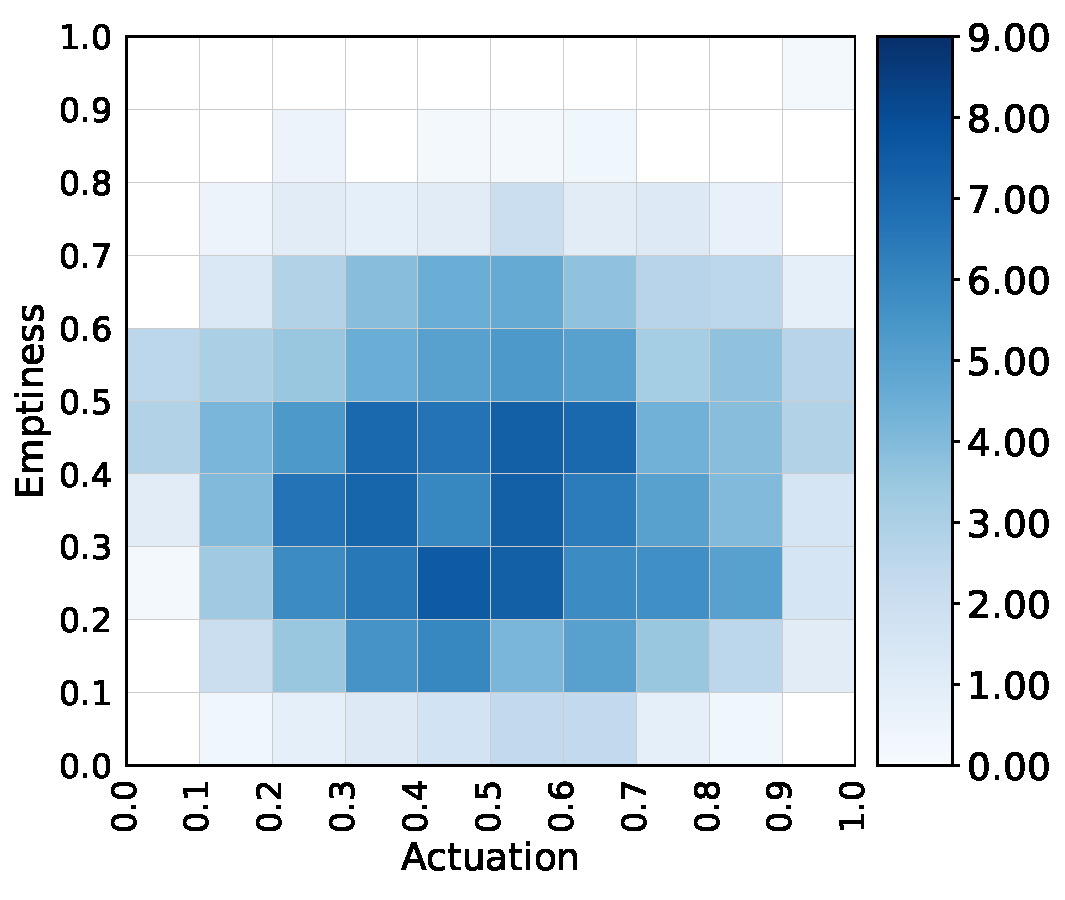
\includegraphics[scale=0.45]{images/brain_opt/walker/walker_qd_40eps_ag}
         \caption{40 episodes}
         \label{walker_ag_40}
    \end{subfigure}
    \hfill
    \begin{subfigure}[b]{0.49\textwidth}
         \centering
         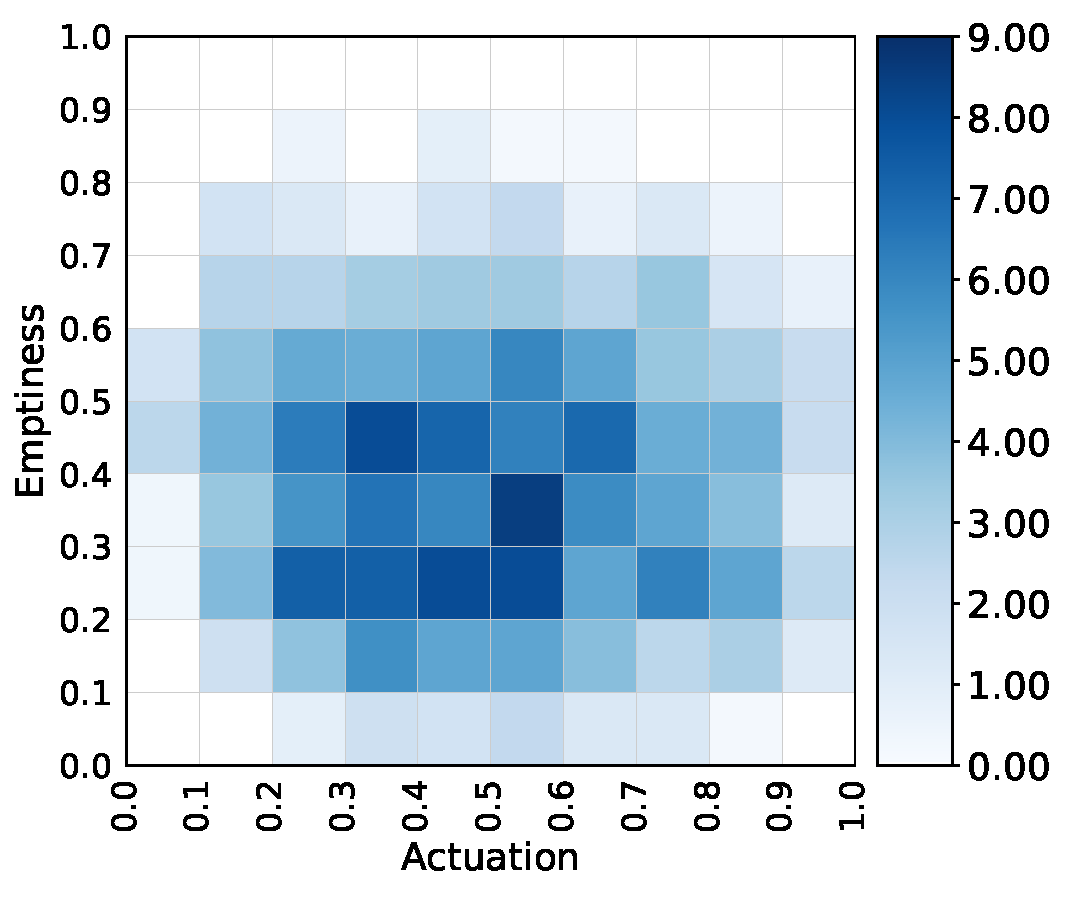
\includegraphics[scale=0.45]{images/brain_opt/walker/walker_qd_60eps_ag}
         \caption{60 episodes}
         \label{walker_ag_60}
    \end{subfigure}
    \caption{Comparison of the activity maps applying controller optimization using 40 (a) or 60 (b) episodes. The overall distribution of the visited bins is not affected.}
    \label{fig:activity_map}
\end{figure}

\begin{figure}[H]
    \centering
    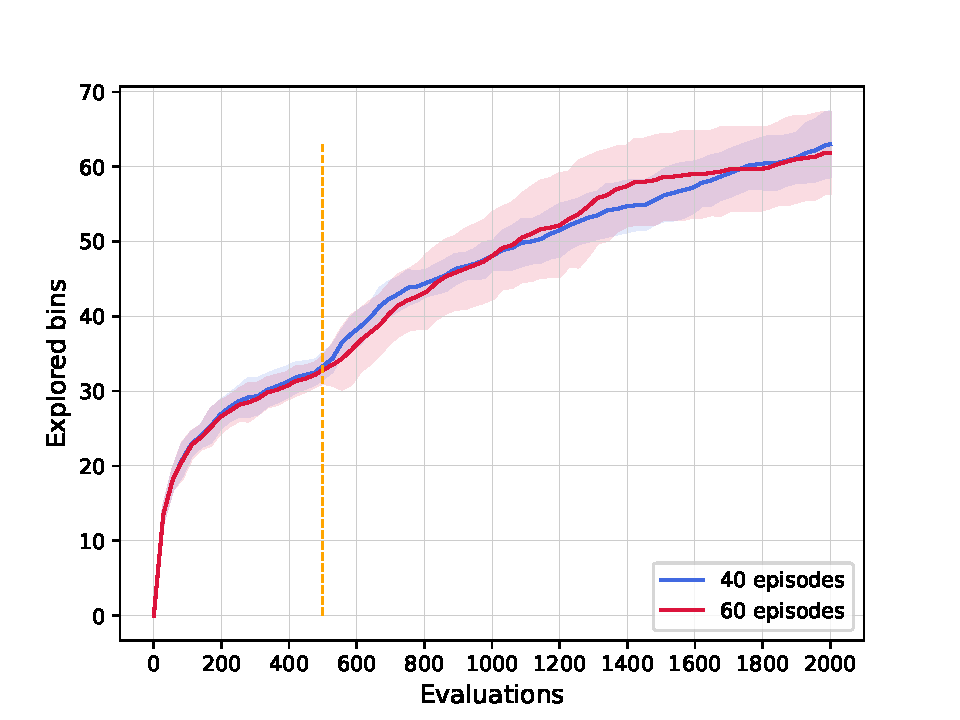
\includegraphics[scale=0.65]{images/brain_opt/walker/comp_40_60eps_at}
    \caption{Comparison of the activity trends. Changing the number of episodes for the controller optimization does not affect the activity trend, since the choice of individuals to mutate and evaluate doesn't depend on the fitness obtained}
    \label{fig:activity_trend}
\end{figure}

\subsection{Performance}
An analysis on how changing the number of episodes for the controller optimization affects the overall performance is here proposed.\\
A comparison of the fitness trends, that describe the behaviour of the best fitness value found after a certain number of evaluations, is illustrated in Figure \ref{fig:fitness_trend}, and it shows that individuals with a 60-episode-optimized controller obtain a greater reward. What is more, the 40-episodes trend has constantly greater variation, probably because of the intrinsic fitness of some morphologies: the naturally fittest bodies can get a great score even though the controller is not highly optimized, while others need to put more effort on the brain optimization to perform their best.

The effects on the fitness can be also inferred comparing the performance maps, that show for each cell the best fitness value obtained by an individual mapped to that cell; brighter cells are the ones that reached a greater fitness value.
The comparison in Figure \ref{fig:performance_map}, show that optimizing the controller with more episodes leads to greater scores all over the map, resulting in a widely spread brighter color.
This means that the more intensive controller optimization didn't affect a type of individual only, but allowed a general improvement, for all the visited cells, including the border ones.

\begin{figure}[h]
    \centering
    \begin{subfigure}[b]{0.49\textwidth}
         \centering
         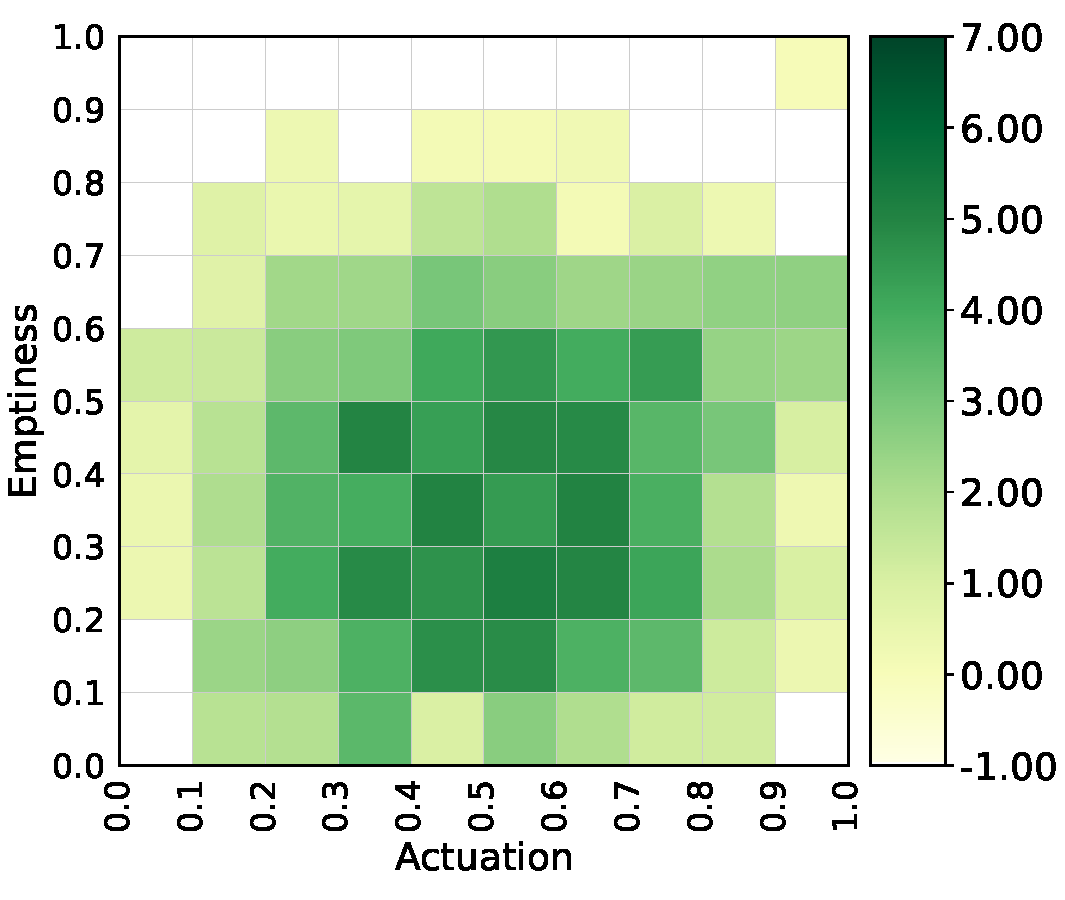
\includegraphics[scale=0.45]{images/brain_opt/walker/walker_qd_40eps_pg}
         \caption{40 episodes}
         \label{walker_pg_40}
    \end{subfigure}
    \hfill
    \begin{subfigure}[b]{0.49\textwidth}
         \centering
         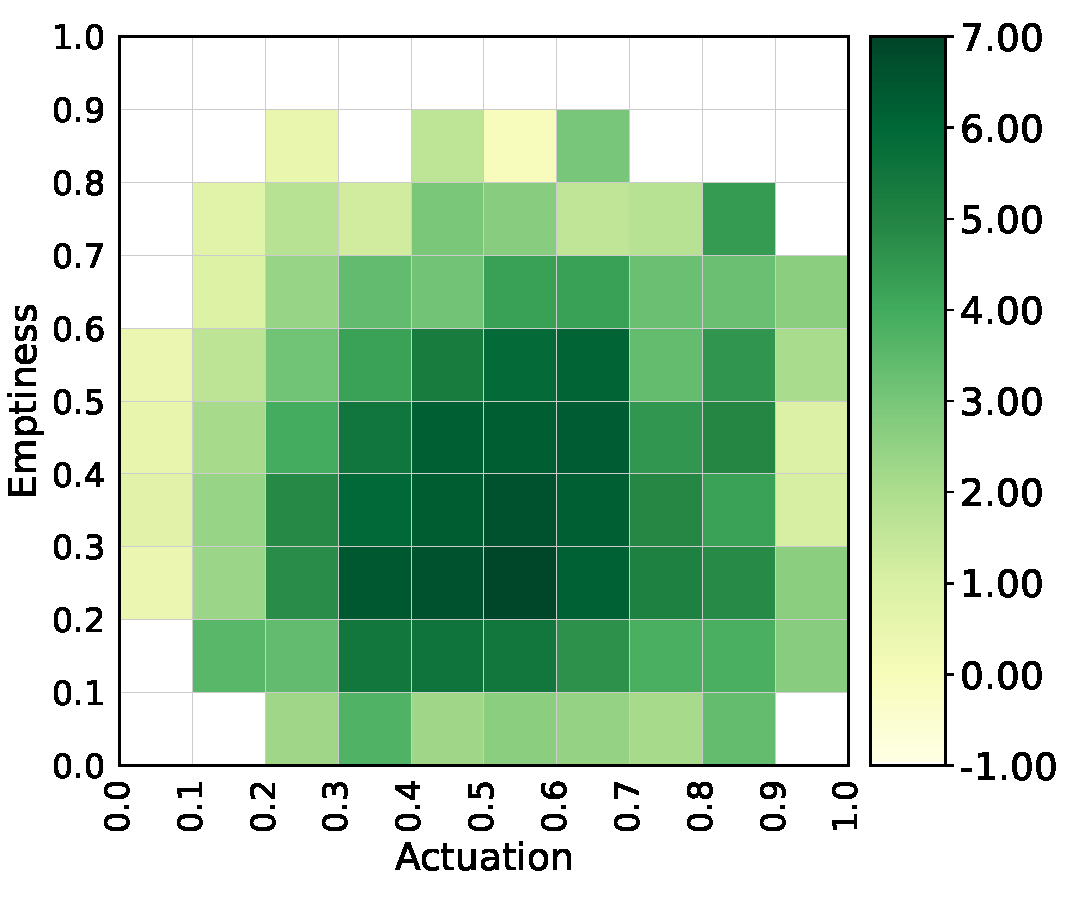
\includegraphics[scale=0.45]{images/brain_opt/walker/walker_qd_60eps_pg}
         \caption{60 episodes}
         \label{walker_pg_60}
    \end{subfigure}
    \caption{Comparison of the performance maps applying controller optimization with 40 (a) or 60 (b) episodes.
    Controller optimization highly affects the general performance of all individuals.}
    \label{fig:performance_map}
\end{figure}

\begin{figure}[h]
    \centering
    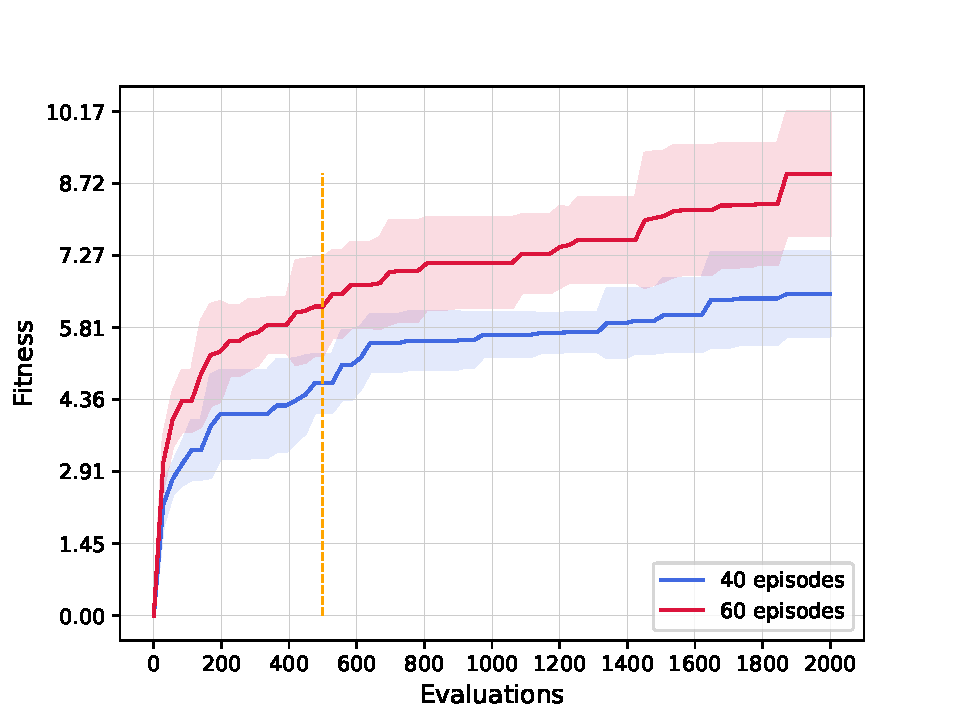
\includegraphics[scale=0.65]{images/brain_opt/walker/comp_40_60eps_ft}
    \caption{Comparison of the fitness trends. A focus on the controller optimization leads to higher fitness.}
    \label{fig:fitness_trend}
\end{figure}


\section{Conclusion}
This experiments confirmed that the controller optimization has a key role in improving the general performance of the individuals and it consequently leads to a greater reward. However, changing the number of episodes for the controller didn't affect the overall exploration of the map, since MAP-Elites chooses the individuals to mutate and evaluate from the ones stored in the map with no regard for their fitness value, as it was expected of a QD algorithm.


\newpage